\section{Results}
\label{sec:results}

The notebook experiments provide exploratory illustrations of the concepts in
Section~\ref{sec:theory}. They were conducted to develop familiarity with SDE
simulation and coefficient estimation, rather than to establish a general
benchmark or a minimum training-data requirement. The main observations concern
the different roles of observation spacing and trajectory duration, and the
limitations of fitting a local transition approximation to coarsely sampled data.

\subsection{Analytic examples and neural SDE setup}
\label{sec:analytic-results}

Brownian motion and the randomly forced harmonic oscillator illustrate the
analytic diffusion estimators in Section~\ref{sec:sde-theory}. The Brownian
example uses a true diffusion amplitude of $0.8$. From the endpoints of 300
independent paths at $T=40$, the variance-based formula
$\widehat{\sigma}=\sqrt{\frac{1}{NT}\sum_j(X_T^{(j)})^2}$ gives $0.8111$.
Fitting a normal distribution to these endpoints using SciPy's
\texttt{norm.fit}, with its mean fixed at zero, and dividing the fitted
standard deviation by $\sqrt{T}$ gives the same value. These are two ways of
calculating the endpoint estimator in
Equation~\eqref{eq:brownian-endpoint-mle}.

The estimate $0.8028$ instead uses all 2,000 increments of the last path,
with spacing $h=0.02$. It is calculated as
$\widehat{\sigma}=\sqrt{\frac{1}{mh}\sum_i(\Delta X_i)^2}$, following
Equation~\eqref{eq:brownian-increment-mle}. This also uses the known zero
mean and the variance identity, applied to increments rather than endpoints.
The two reported values therefore differ because they use different data
summaries, rather than because one uses SciPy and the other uses variance.

For the oscillator, corrected totals give
$0.2596$, whereas pooled drift-corrected velocity increments give $0.3000024$
for a true amplitude of $0.3$. These are individual simulated datasets using
different observation summaries; the estimates illustrate the calculations
without establishing a general accuracy ranking.

\label{sec:neural-results}
The neural example uses the periodic-potential SDE
\begin{equation}
    dX_t=-\sin(X_t)\,dt+1.1\,dW_t,\qquad X_0=0.
\end{equation}
The model learns a periodic drift function and a positive constant diffusion
using the local Gaussian loss in Equation~\eqref{eq:neural-sde-nll}.
The comparisons below use 50 training trajectories, simulated over $T=500$
with 15,000 saved observations per path. The saved spacing is approximately
$0.03334$, with four Euler integration steps per observation interval.
Subsampling or truncating these paths changes the observation spacing or
duration while preserving the underlying numerical simulation.

Each configuration is fitted five times with new training data and training
seeds. Configurations within a repeat share the training pool and seed.
Training uses Adam with learning rate $10^{-3}$, minibatches of 2,048
increments, and 1,500 updates. Checkpoints are selected using a fixed sample
of 4,096 held-out increments at the original fine observation spacing,
including the untrained model as a candidate. Coefficient errors follow
Equation~\eqref{eq:coefficient-errors}, with drift evaluated on 512 uniformly
spaced points over one period. The figures report medians and interquartile
ranges across five fits; the bands describe variation between runs, rather
than confidence intervals.

\subsection{Observation spacing and diffusion recovery}
\label{sec:data-size-results}

At fixed duration $T=500$, increasing the number of observations per path
reduces the distance in time between observations.
Figure~\ref{fig:repeated-density} shows that median diffusion error decreases
from $18.18\%$ at spacing $\Delta t\approx1.00$ to $0.86\%$ at
$\Delta t\approx0.03334$. Drift error initially improves as the coarsest
sampling is refined, but does not continue to decrease with denser sampling:
its median is $8.45\%$ at 3,000 observations and $10.72\%$ at 15,000.
Thus, once the coarsest intervals are excluded, finer sampling benefits
diffusion recovery more consistently than drift recovery in this example.

\begin{figure}[htbp]
    \centering
    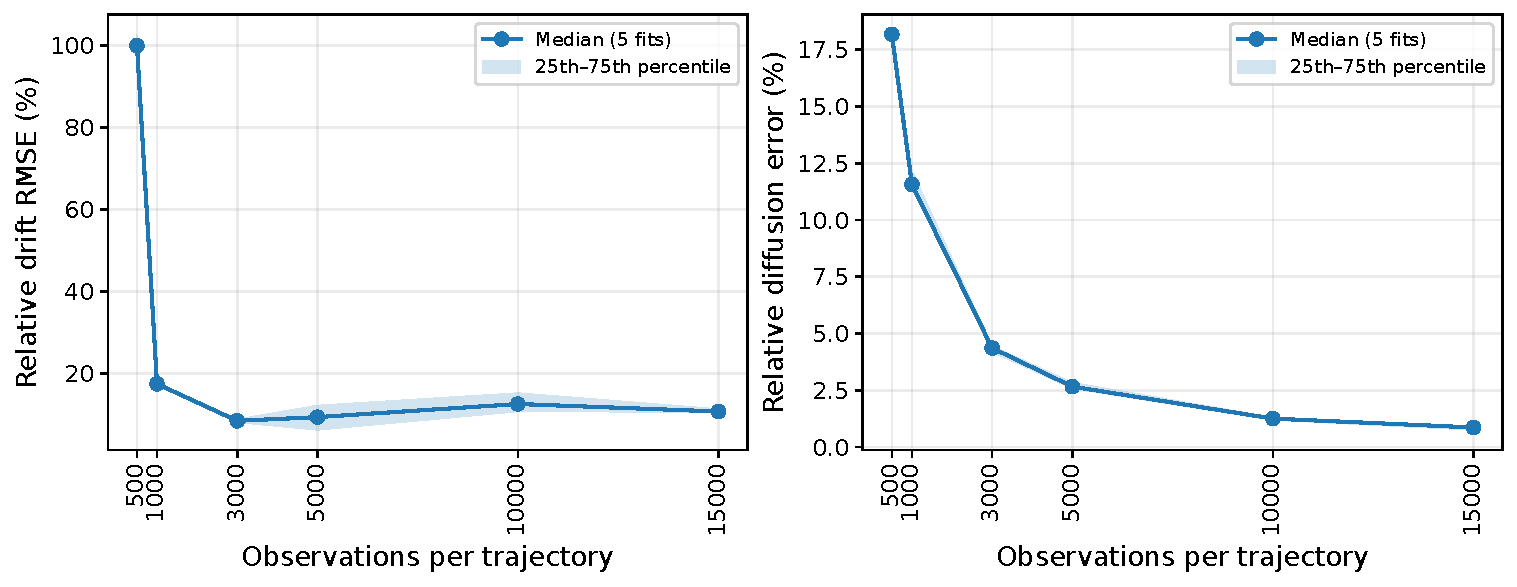
\includegraphics[width=0.9\linewidth]{figures/results/repeated-observation-density.pdf}
    \caption{Exploratory observation-density sweep at fixed duration $T=500$
    with 50 training trajectories. Lines show median coefficient errors over
    five fits; bands show the 25th--75th percentiles. Validation uses the
    original fine observation spacing for every configuration.}
    \label{fig:repeated-density}
\end{figure}

This distinction is consistent with the local increment model in
Equation~\eqref{eq:local-gaussian}: the drift contribution scales with
$\Delta t$, while the random contribution scales with $\sqrt{\Delta t}$.
Reducing the interval therefore makes the drift contribution smaller relative
to the noise in each increment. More frequent observations over the same time
span need not improve drift recovery in the same way as diffusion recovery.

\subsection{Trajectory duration and drift recovery}

The duration comparison keeps observation spacing approximately $0.03334$
and uses progressively longer prefixes of the same paths.
In Figure~\ref{fig:repeated-duration}, median drift error decreases overall
from $17.08\%$ at $T\approx33.30$ to $10.72\%$ at $T=500$, although the
intermediate values fluctuate. Diffusion error is already small at the
shortest duration: its median changes from $1.11\%$ to $0.86\%$ between
these endpoints.

\begin{figure}[htbp]
    \centering
    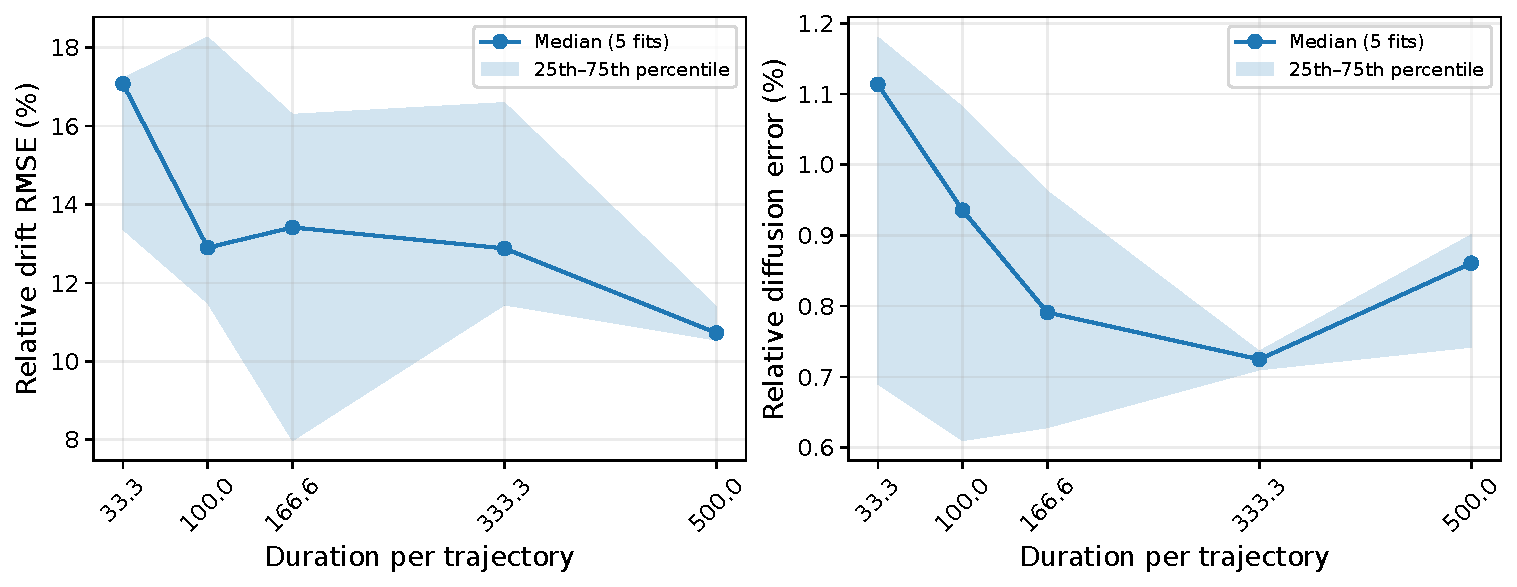
\includegraphics[width=0.9\linewidth]{figures/results/repeated-duration.pdf}
    \caption{Exploratory duration sweep with 50 training trajectories and
    fixed observation spacing $\Delta t\approx0.03334$. Lines show median
    coefficient errors over five fits; bands show the 25th--75th percentiles.}
    \label{fig:repeated-duration}
\end{figure}

The comparison illustrates why observation spacing and total observation time
should be distinguished. Longer trajectories provide additional time over
which to observe the systematic drift, whereas denser sampling resolves
short-time fluctuations. Here, extending duration gives an overall improvement
in drift recovery that is absent when only the already fine sampling is made
denser. This is an observed tendency, not a monotonic learning curve or a
separation of the two coefficients: both depend on the data and fitting
procedure.

\paragraph{Number of training trajectories.}
A further comparison uses 5, 10, 20, 30, 40, and 50 trajectories, keeping
$T=500$, 15,000 observations per path, and 1,500 updates fixed. Across five
fits per configuration, median drift error decreases from $16.25\%$ with five
paths to $10.72\%$ with 50, but fluctuates between these settings; its lowest
value is $8.34\%$ with 40 paths. Median diffusion error remains below $1\%$
throughout. More trajectories therefore do not consistently reduce the errors
under this fixed training budget.

\paragraph{Number of training updates.}
Full-duration, shorter-duration, and coarse-sampling configurations are also
checked at 1,500, 3,000, and 6,000 updates, using two data/training seed pairs.
Each fit continues along the same training sequence, selecting the best
validation checkpoint available at each budget. More updates do not
consistently improve drift recovery: in one shorter-duration run, selected
drift error changes from $13.41\%$ to $33.33\%$ and then $18.68\%$, despite
small improvements in validation loss. These checks do not establish
convergence at 1,500 updates and show that lower validation loss need not mean
more accurate drift.

\subsection{Coarse sampling and validation at the original scale}

The coarsest configuration exposes a limitation of the fitting approach.
With 500 observations over $T=500$, training intervals are approximately
$1.00$, while validation intervals remain approximately $0.03334$.
Four of the five fits select the untrained initial checkpoint: none of their
evaluated trained checkpoints improves its fine-scale validation loss.
The selected diffusion remains at its initial value $0.9$, giving
$18.18\%$ error relative to the true amplitude $1.1$. Two extended checks
still select the untrained checkpoint after 6,000 updates. In this specific
validation sense, the untrained model performs better than the evaluated
trained models, despite having inaccurate coefficients itself.

A plausible explanation is the mismatch between a local Gaussian transition
model and increments spanning a long interval. The loss approximates the drift
and diffusion as constant within each interval. Over a coarse interval, the
state can move through regions with different drift, so the observed
displacement combines dynamics that this approximation does not resolve.
Fitting it can therefore favor coefficients that represent finite-interval
transitions rather than the original instantaneous SDE coefficients. Such a
representation need not transfer to the original fine time scale used for
validation. Coarse sampling leaves the generating SDE unchanged, but obscures
the within-interval dynamics in the observations used by this loss.

The checkpoint results demonstrate the failure to improve fine-scale
validation in these runs. They are consistent with this approximation-error
explanation, but do not isolate it from optimization effects or establish that
the trained models accurately fit the coarse transitions. The practical lesson
of these exploratory examples is that observation spacing, trajectory duration,
and the time scale assumed by the loss all matter when interpreting learned
SDE coefficients. Full experiment details and outputs remain in
\texttt{likelihood\_calc.ipynb}, \texttt{sde\_test\_data.ipynb}, and
\texttt{sandbox/experiment\_results}.
